%%%%%%%%%%%%%%%%%%%%%%%
% trigger and datasets 
%%%%%%%%%%%%%%%%%%%%%%%

\subsection{Data and trigger \label{sec:boost_data_trigger}}

The analysis presented in this thesis is based on 19.7\fbinv of 8\TeV proton-proton collision data
collected by the CMS experiment in 2012.  The data are divided into four data taking periods
(A, B, C, and D) to deal with changing conditions such as the average pileup or peak luminosity. 
Events used in the razor boost analysis are selected using two triggers from the CMS high
level trigger system (see Section~\ref{sec:cms_hlt}), requiring either the highest jet \pt or the
scalar sum of jet transverse momenta, $\HT$, to be above certain thresholds. 
The jet \pt trigger, of which the different implementations are denoted by \texttt{PFJet*},
had a threshold on the \pt of the highest \pt jet of 320\GeV for most of the runs, and a threshold
of 400\GeV for a short period. 
The $\HT$-based trigger, denoted by \texttt{PFHT*}, had an $\HT$ threshold of 650\GeV. 
The two trigger algorithms were based on a fast implementation of the particle flow 
reconstruction method, which was described in Section~\ref{sec:event_reco_pf}.  
The exact names of the trigger used by run are given in Table~\ref{tab:boost_triggers}. The primary
datasets which include the data collected by these triggers are listed in
Table~\ref{tab:boost_primary_datasets}. 

\begin{table}[htdp]
\caption{Summary of HLT triggers that are used in this analysis. Events in a given run range
are selected if they pass at least one of the listed triggers. }	
\begin{center}
\begin{tabular}{l l l l}
\toprule
Period & Run range & PFJet HLT & PFHT HLT \\
\midrule
\multirow{3}{*}{Run2012A} & 190456 - 190738 & PFJet320\_v3 & PFHT650\_v5 \\
& 190762 - 191426 & PFJet320\_v4 & PFHT650\_v6 \\
& 191512 - 193686 & PFJet320\_v5 & PFHT650\_v7 \\
\midrule
\multirow{2}{*}{Run2012B} & 193746 - 196027 & PFJet320\_v5 & PFHT650\_v8 \\
& 196039 - 197722 & PFJet320\_v5 & PFHT650\_v9 \\
\midrule
\multirow{3}{*}{Run2012C} & 197770 - 199631 & PFJet400\_v6 & PFNoPUHT650\_v1 \\
& 199648 - 202585 & PFJet320\_v8 & PFNoPUHT650\_v3 \\
& 202807 - 203734 & PFJet320\_v9 & PFNoPUHT650\_v4 \\
\midrule
Run2012D & 203754 - 208940 & PFJet320\_v9 & PFNoPUHT650\_v4 \\
\bottomrule
\end{tabular}
\end{center}
\label{tab:boost_triggers}
\end{table}

\begin{table}[htdp]
\caption{List of primary datasets and corresponding run ranges, containing data for a total
integrated luminosity of $19.712\fbinv$.}
\begin{center}
\begin{tabular}{ l l }
\toprule
Primary dataset & Run range \\
\midrule
/Jet/Run2012A-22Jan2013-v1/ & 190456 - 193621 \\
/HT/Run2012A-22Jan2013-v1/  & 190456 - 193621 \\
/JetHT/Run2012B-22Jan2013-v1/ & 193833 - 196531 \\
/JetHT/Run2012C-22Jan2013-v1/ & 198022 - 203742 \\
/JetHT/Run2012D-22Jan2013-v1/ & 203777 - 208686  \\
\bottomrule
\end{tabular}
\end{center}
\label{tab:boost_primary_datasets}
\end{table}

\begin{table}[htdp]
\caption{List of primary datasets used to measure the trigger efficiency. }
\begin{center}
\begin{tabular}{ l l }
\toprule
Primary dataset & Run range \\
\midrule
/SingleElectron/Run2012A-22Jan2013-v1/ & 190456 - 193621 \\ 
/SingleElectron/Run2012B-22Jan2013-v1/ & 193833 - 196531 \\
/SingleElectron/Run2012C-22Jan2013-v1/ & 198022 - 203742 \\
/SingleElectron/Run2012D-22Jan2013-v1/ & 203777 - 208686  \\
\midrule
/SingleMu/Run2012A-22Jan2013-v1/ & 190456 - 193621 \\ 
/SingleMu/Run2012B-22Jan2013-v1/ & 193833 - 196531 \\
/SingleMu/Run2012C-22Jan2013-v1/ & 198022 - 203742 \\
/SingleMu/Run2012D-22Jan2013-v1/ & 203777 - 208686 \\
\bottomrule
\end{tabular}
\end{center}
\label{tab:boost_primary_datasets_trigeff}
\end{table}

In order to select events with unbiased jet \pt and $\HT$ distributions,
the trigger efficiency was measured from a sample of events collected with an orthogonal set of
triggers requiring at least one electron or muon. The corresponding primary datasets are listed in
Table~\ref{tab:boost_primary_datasets_trigeff}. 
The trigger efficiency $\epsilon_\textrm{trig}$ is determined as a function of $\HT$ and first jet
\pt, and takes as basis for the measurement the baseline selection described further in
Section~\ref{sec:boost_baseline_selection},
\begin{equation}
  \epsilon_\textrm{trig} = \frac{\textrm{Events passing baseline and trigger selection}}
{\textrm{Events passing baseline selection}}.
\end{equation}
It was checked that the trigger efficiency obtained from either the electron or muon sample gives 
consistent results. Both samples were combined to derive the final trigger efficiency measurement in 
order to increase the statistical precision.
Figure~\ref{fig:boost_trigger_efficiency} shows, on the top plot, the trigger efficiency
measured from data on the ($\HT$, first jet \pt) plane.
We observe that the trigger is fully efficient for events with $\HT > 800\GeV$.  
In order to account for the lower efficiency of the region with $\HT  < 800\GeV$, the measured
trigger efficiency over the ($\HT$, first jet \pt) plane is applied as an event-by-event weight
to the simulated samples. The bottom plot of Fig.~\ref{fig:boost_trigger_efficiency} shows the
effect of this trigger efficiency across the (\mr,\rsq) plane for the total simulated background. 
The uncertainty in the trigger efficiency is taken to be the maximum of the statistical 
uncertainty, and the difference in trigger efficiency obtained using the baseline selection and no 
selection at all. As the uncertainties are not symmetric, we show both the up and down uncertainties
in Fig.~\ref{fig:boost_trigger_efficiency_unc}. They are generally below 5\%.   


\begin{figure}[p]
\centering
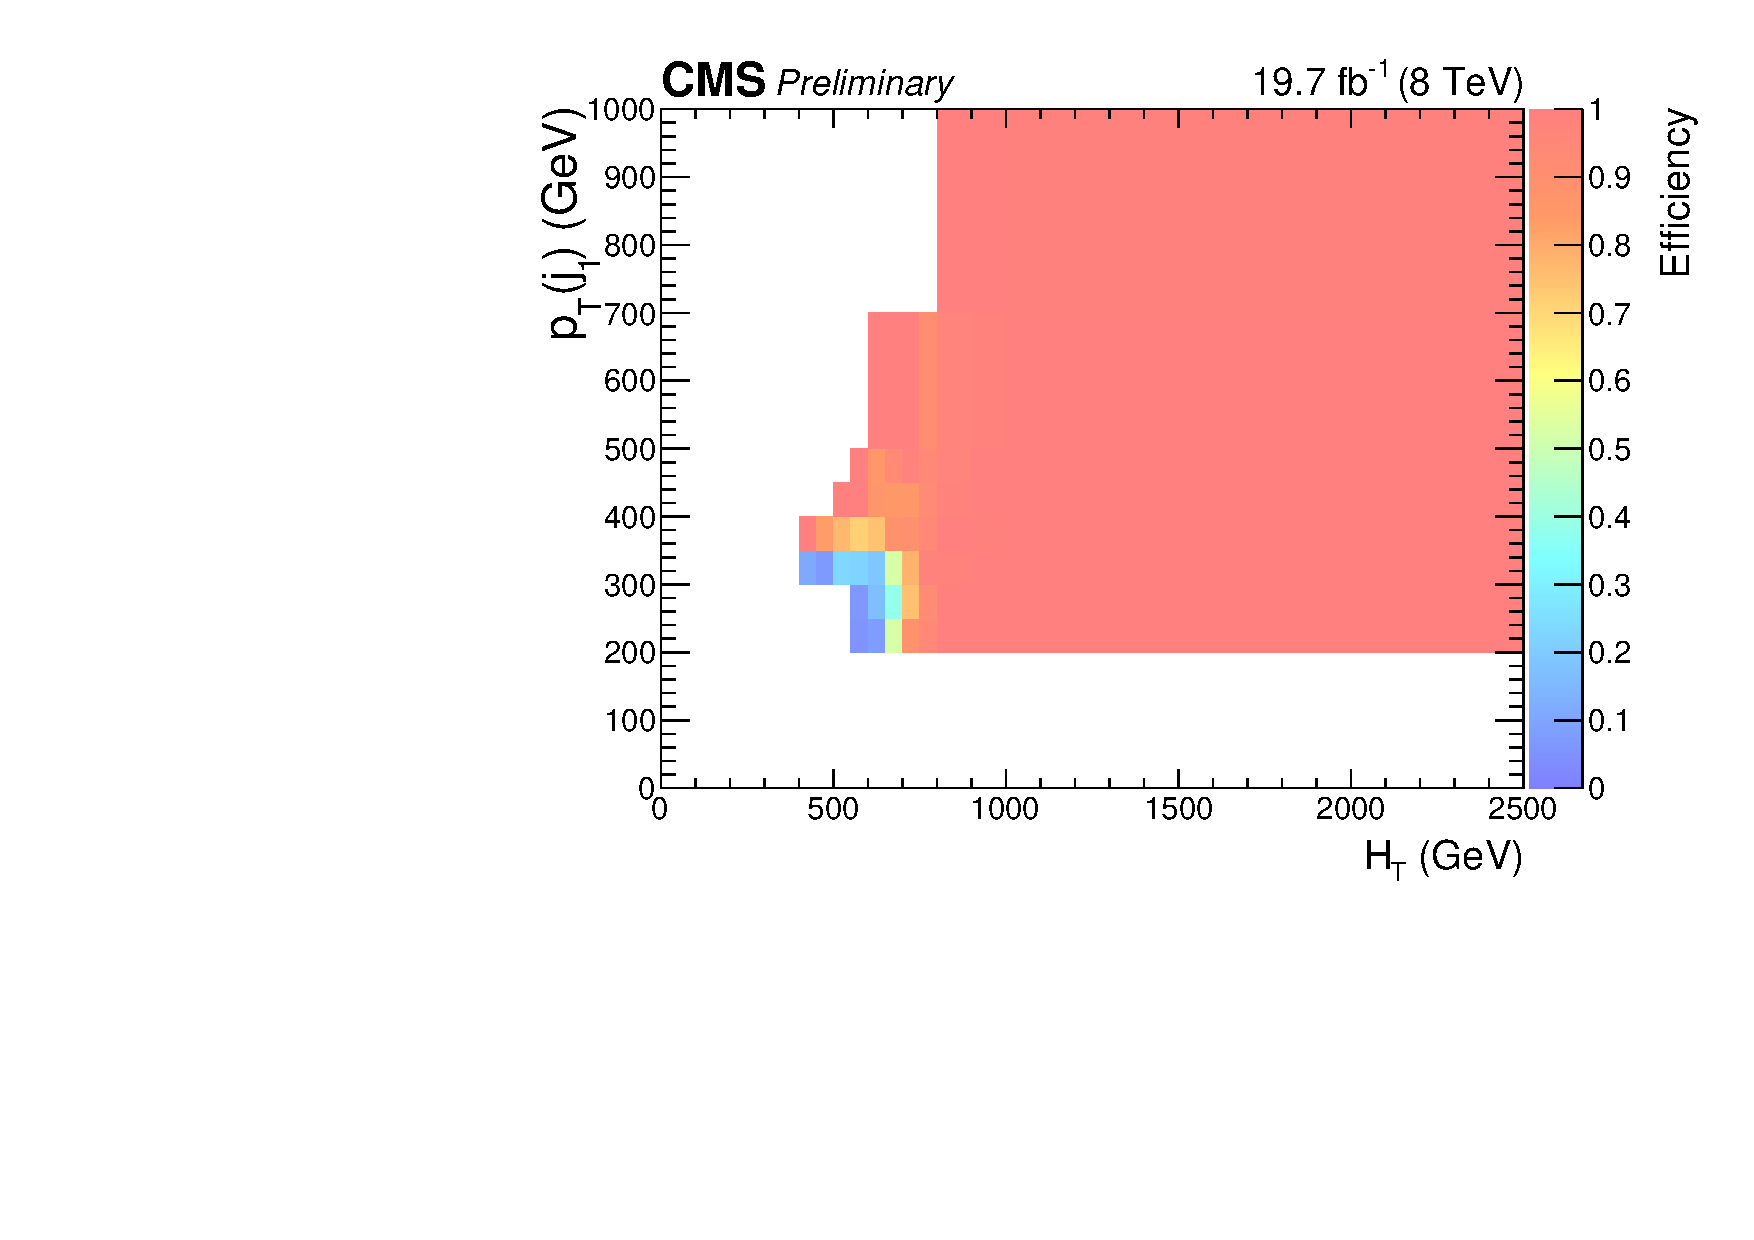
\includegraphics[width=0.9\textwidth]{figures/razor_trigger/h_HT_j1pt_pre_eff_ph_l}

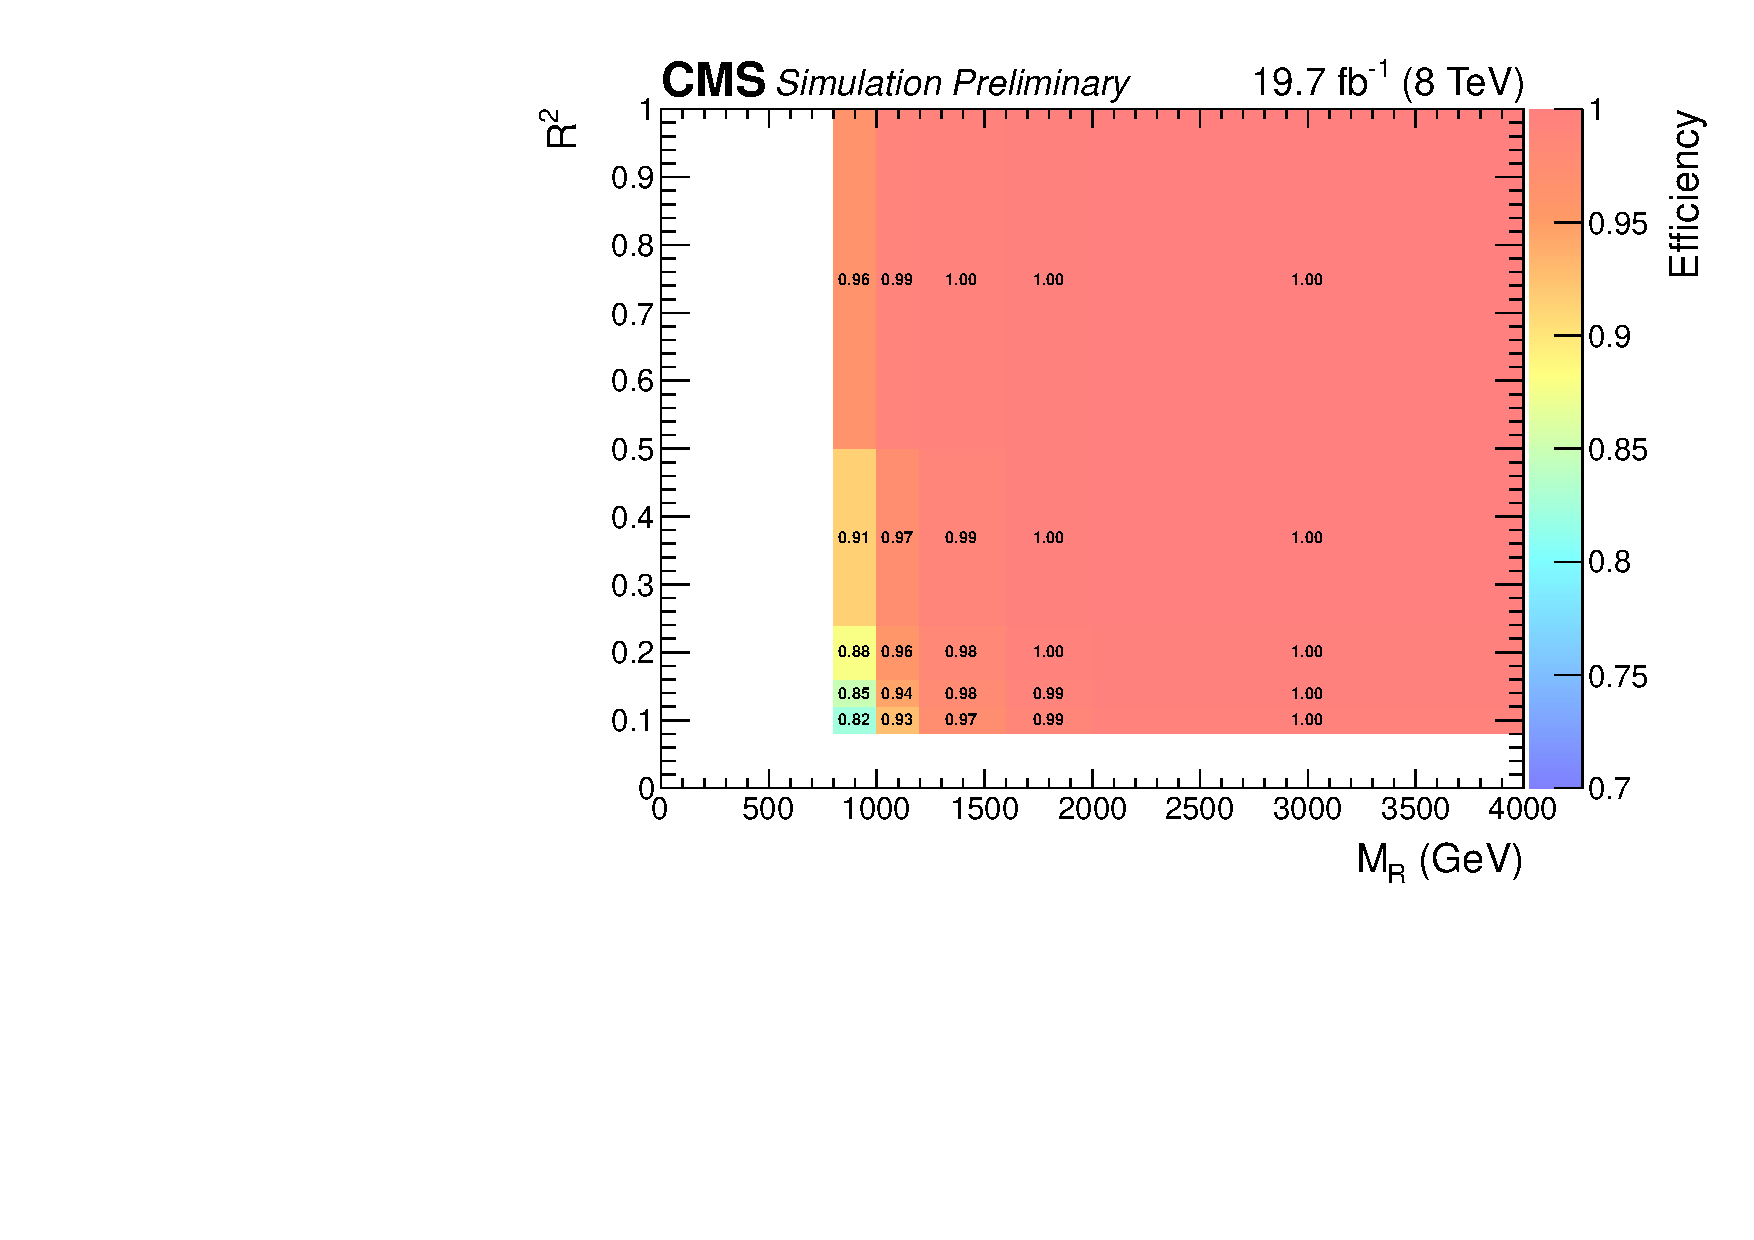
\includegraphics[width=0.9\textwidth]{figures/razor_trigger/MR_R2_bg_trig_eff}
\caption{[top] The trigger efficiency, obtained from data, as a function of $H_T$ and first jet
$\pt$ after the preselection mentioned in Section~\ref{sec:boost_baseline_selection}.
[bottom] The trigger efficiency as a function of $\mathrm{M_R}$ and $\mathrm{R^2}$ after the same
preselection, obtained by applying the trigger efficiency as a function of $\HT$ and first jet $\pt$
to the total simulated background. 
\label{fig:boost_trigger_efficiency}}
\end{figure}  

\begin{figure}[htpb]
\centering
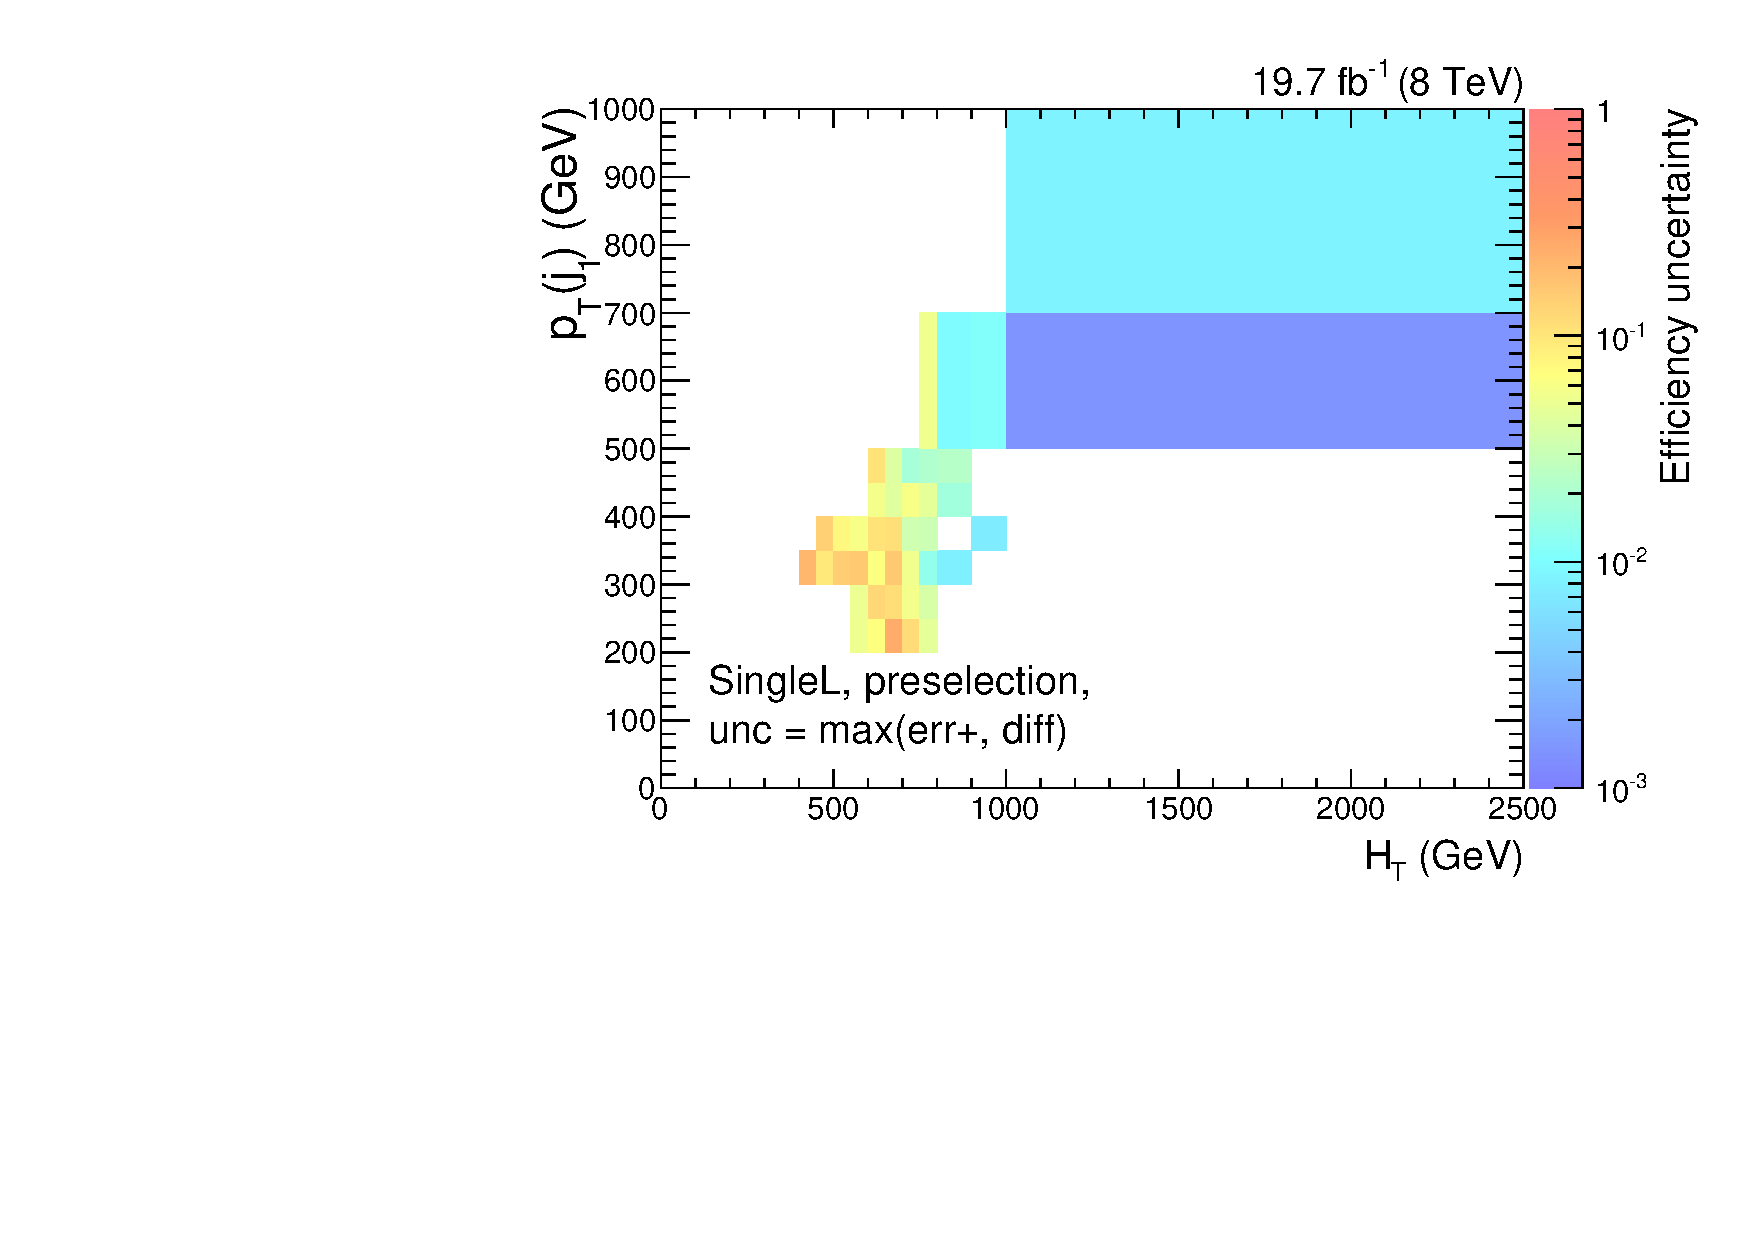
\includegraphics[width=0.48\textwidth]
{figures/razor_trigger/h_HT_j1pt_0_pre_errdiff_up_ph_l_forThesis}
~
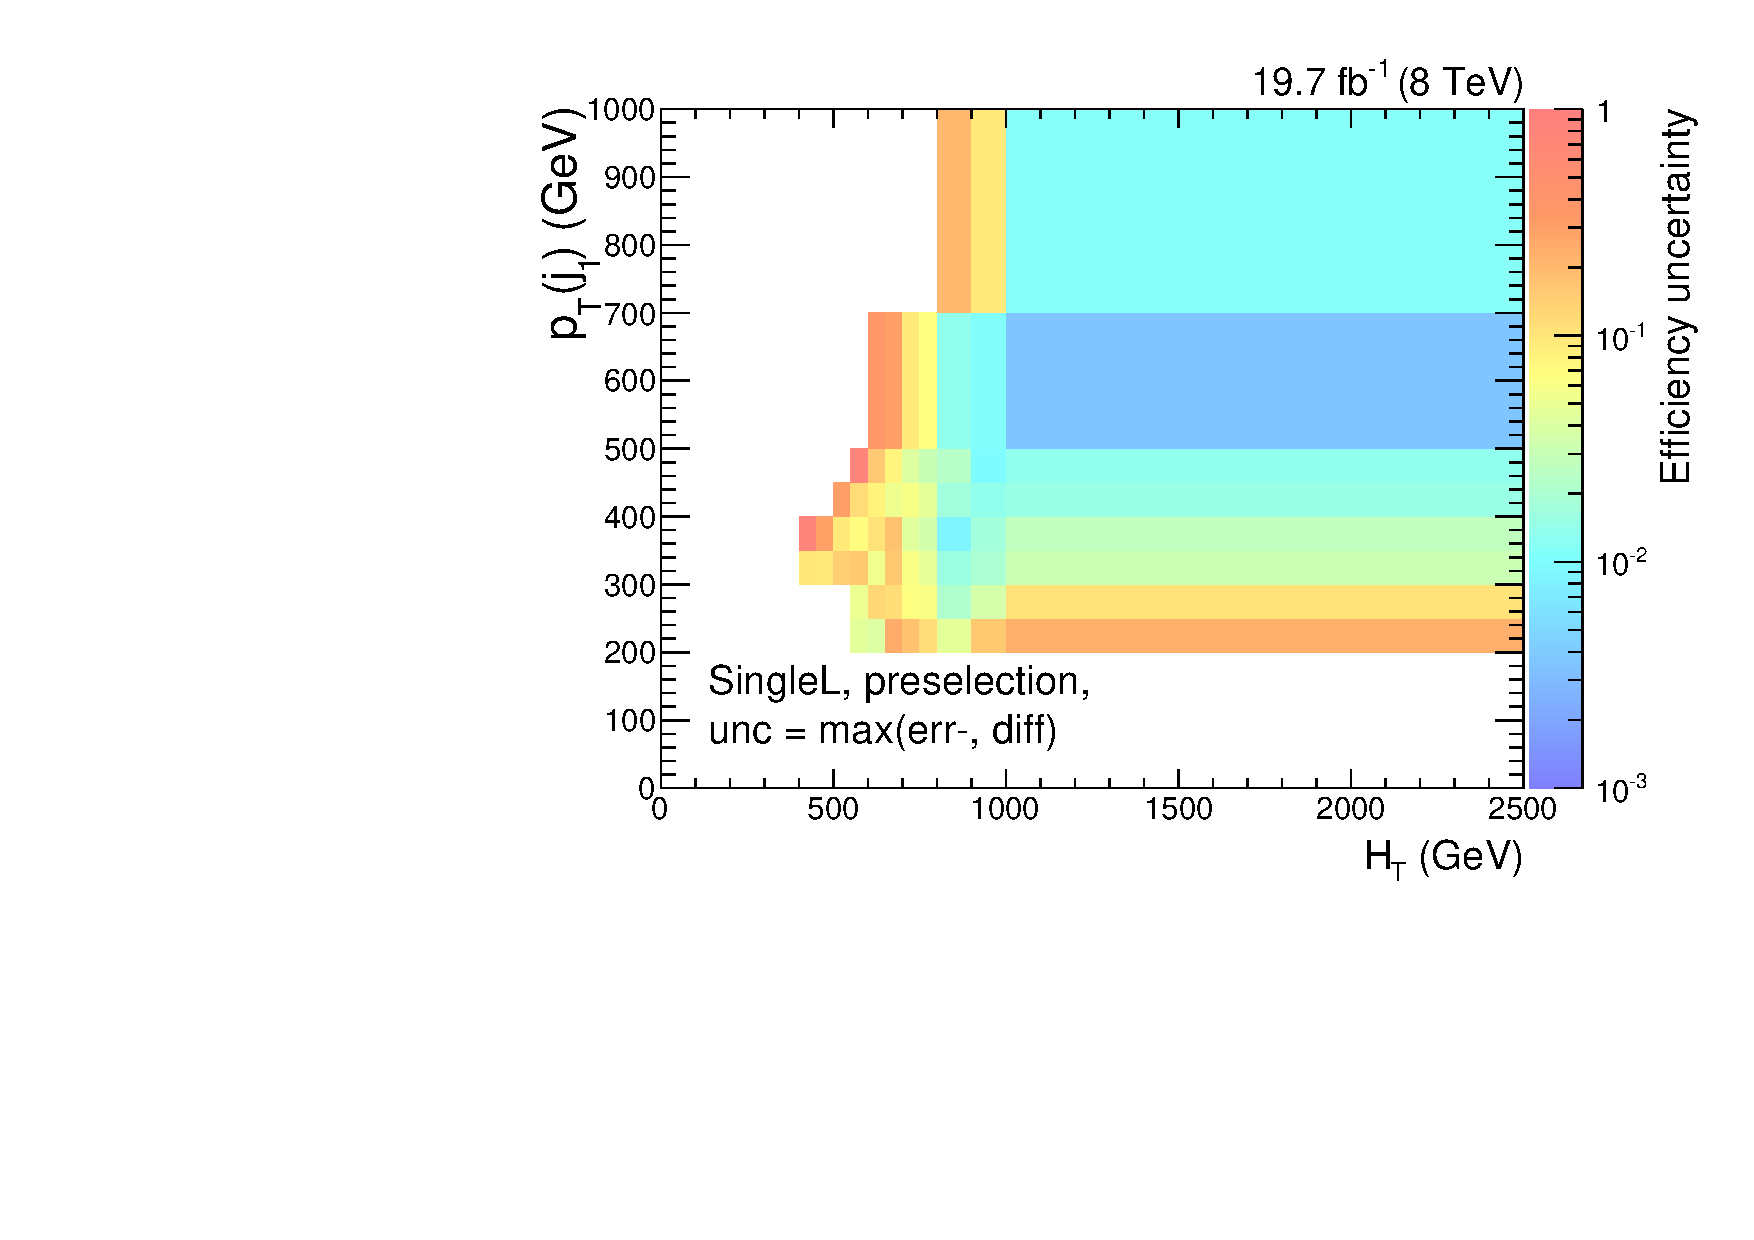
\includegraphics[width=0.48\textwidth]
{figures/razor_trigger/h_HT_j1pt_0_pre_errdiff_low_ph_l_forThesis}
\caption{The magnitude of the up (left) and down (right) uncertainties on the efficiency as 
functions of $\HT$ and first jet $\pt$, obtained using the combination of the SingleEle and SingleMu 
datasets. 
\label{fig:boost_trigger_efficiency_unc}}
\end{figure}



%%%%%%%%%%%%%%%%%%%%%%%%%%%%%%%%%%%%%%%%%%%%%%%%%%%%%%%%%%%%%%%%%%%%%%%%%%%%%%%%%%%%%%%%%%%%%%%%%%%%
\subsection{Simulated samples \label{sec:boost_mc_samples}}

The simulated samples are used to investigate the characteristics of the background and signal
processes.  The complete list of simulated samples that are used in the analysis is given in
Appendix~\ref{app:datasets}, in Tables~\ref{tab:boost_mc_bg} and \ref{tab:boost_mc_bg2} for the SM
background samples, and in Table~\ref{tab:boost_mc_sms} for the signal samples. 

Multijet, $t\bar{t}$, $\W({\rightarrow}\,\ell\nu)+$jets, $\cPZ/\gamma^*({\rightarrow}\,
\ell\bar{\ell})+$jets, and $\cPZ({\rightarrow}\, \nu \bar{\nu})+$jets events are generated using
\MADGRAPH 5.1.3.30~\cite{Alwall:2011uj}, as are the smaller backgrounds $\W({\rightarrow}\, q
\bar{q})bb$, 
$\W\W\cPZ+$jets, $\W\W\gamma+$jets, $\cPZ\cPZ\cPZ+$jets, $t\bar{t}\gamma+$jets, and
$t\bar{t}\W\W+$jets.
Events for the $\cPZ/\gamma^*({\rightarrow} c\bar{c})$, $\cPZ/\gamma^*({\rightarrow}
\cPqb\bar{\cPqb})$,
$\W\W$, $\W\cPZ$, and $\cPZ\cPZ$ processes are generated using 
{\PYTHIA}6.424~\cite{Sjostrand:2006za}.
For all these samples CTEQ6L1~\cite{Pumplin:2002vw} is used as the set of parton distribution
functions. 
Single top quark events are generated using \POWHEG 1.0~\cite{powheg,powheg2} with CT10
PDFs~\cite{Lai:2010vv}, and $\W\W\W$, $\W\cPZ\cPZ$, $t\bar{t}\W$ and $t\bar{t}\cPZ$ are generated using
\AMCATNLO~\cite{Frixione:2002ik} with CTEQ6M PDFs~\cite{Pumplin:2002vw}. 
Signal events are produced using \MADGRAPH 5.1.5.4 with CTEQ6L1 PDFs.  

The parton level events are showered and hadronized using {\PYTHIA}6.426 with tune
Z2*~\cite{Chatrchyan:2013gfi}, except for the samples generated with \AMCATNLO which use 
\HERWIG~\cite{Corcella:2000bw,Corcella:2002jc} for the parton shower and hadronization.  
The \MADGRAPH samples are matched to the parton shower using the MLM technique, as discussed
in Section~\ref{sec:event_matching}.
For the background events, the response of the CMS detector is
simulated with a full simulation based on \GEANTfour~\cite{G4}.  
A parameterized fast detector simulation, \ie FastSim (Section~\ref{subsec:fastsim}), is used to
simulate the detector response to the signal events. 


